% !TEX root = ../main.tex
\subsection{FMT Alignment}
\label{ssec::fmt_alignment}
% --+ Why is it needed +--------------------------------------------------------
    In an ideal scenario, the target and each detector would be installed precisely in their required positions.
    However, in the real world, there are inevitable misalignments in their placements.
    These misalignments must be accounted for and incorporated into the reconstruction process to ensure meaningful results.

    Within the CLAS collaboration, the Calibration and Commissioning group (CalCom) is responsible for the alignment and calibration of each detector.
    The shifts and rotations necessary for alignment are included in the Calibration and Conditions Database (CCDB), which is then utilized during reconstruction.

    The alignment work aimed to achieve three primary goals.
    Firstly, to provide FMT alignment tables to Run Group F (RG-F) for use in reconstruction.
    Secondly, to assess whether the resolution improvement obtained from the FMT justifies the additional material introduced into the CLAS12 detector.
    Lastly, to offer detailed information about these improvements, enabling Run Group E (RG-E) and other run groups to make informed decisions on whether to include the detector in their runs.

% --+ Definitions +-------------------------------------------------------------
    Alignment shifts can be performed in any of the three global axes: $z$, which is aligned with the beamline; $x$, which runs parallel to the ground; and $y$, which points upwards from the ground.
    Additionally, alignment rotations can be carried out around these axes.
    Specifically, for the purposes of this work, rotations around the $z$ axis are referred to as $\phi$ rotation (roll), while rotations around the $x$ and $y$ axes are termed pitch and yaw, respectively.

    To quantify misalignment, the DOCA between a reconstructed DC track and an FMT cluster is defined as a \textbf{Residual}.
    Due to the geometry of each layer (as depicted in figure \ref{fig::fmt_geometry}), only the residuals in the local $y$ axis of a layer (perpendicular to the strips) can be measured.
    This implies that global $z$ and $\phi$ alignment can be performed independently for each layer.
    However, global $x$, global $y$, pitch, and yaw alignment must be carried out simultaneously for the entire detector.

% --+ How was it done +---------------------------------------------------------
    \begin{figure}[b!]
        \centering\frame{
        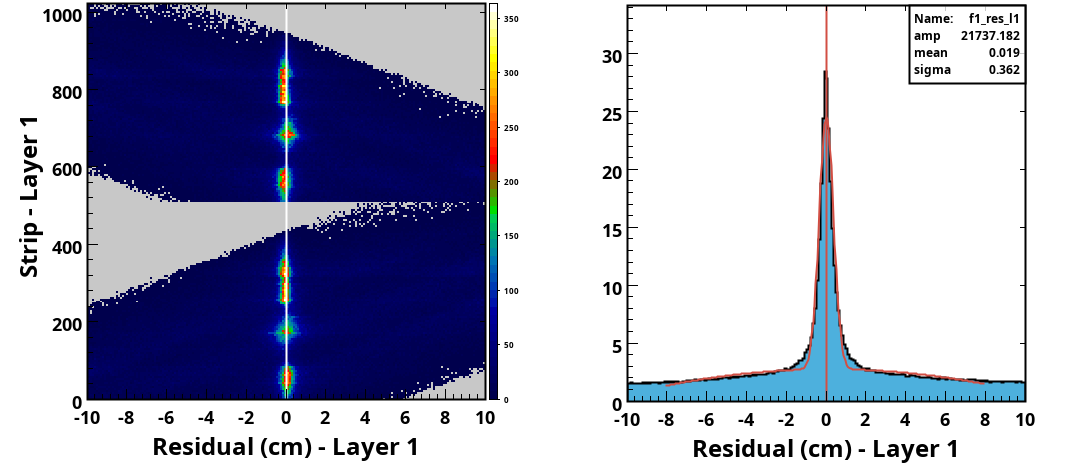
\includegraphics[width=\textwidth]{20res_example.png}}
        \caption[Example FMT residuals plot]{Example FMT residuals plot.
        Source: \hyperlink{github.com/JeffersonLab/clas12alignment}{CLAS12 alignment software}.}
        \label{fig::res_example}
    \end{figure}

    To minimise residuals, they are plotted for a specific shift or rotation in the relevant axes.
    An example of such a plot is illustrated in figure \ref{fig::res_example}.
    Since the residuals are expected to follow a Gaussian distribution, a Gaussian fit is applied to them.

    For $z$ and $\phi$ alignment, the goodness of fit is heuristically evaluated by comparing the standard deviation ($\sigma$) of the Gaussian fits and selecting the shift with the smallest $\sigma$.
    For $x$, $y$, pitch, and yaw alignment, the goodness of fit is heuristically evaluated by choosing the fit with the mean closest to zero.
    It is important to consider a reasonable error margin when selecting the minima.

    Examples of the distributions of goodness of fit for $z$ and $xy$ alignment can be observed in figure \ref{fig::resfit_example}.

    \begin{figure}[t!]
        \centering\frame{
        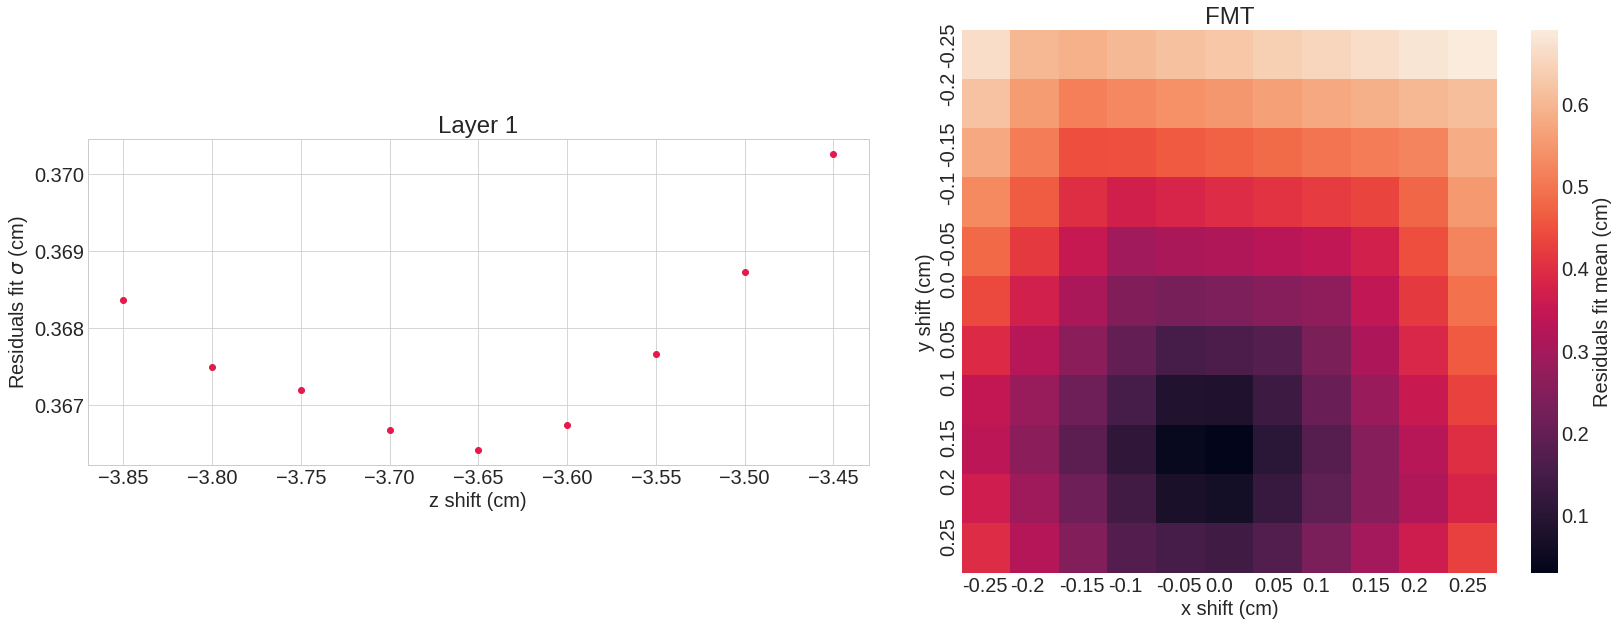
\includegraphics[width=\textwidth]{20resfit_example.png}}
        \caption[Examples of residuals goodness of fit plots]{Examples of residuals goodness of fit plots.
        Source: \hyperlink{github.com/JeffersonLab/clas12alignment}{CLAS12 alignment software}.}
        \label{fig::resfit_example}
    \end{figure}

    % !TEX root = ../main.tex
\subsubsection{Fiducial Cuts}
\label{12.21::fiducial_cuts}
    To mitigate background noise, fiducial cuts are applied to the DC tracks and FMT clusters.
    This process enhances data quality, ensuring more meaningful alignment results.

    For DC tracks, the following cuts are implemented:
    \begin{itemize}
        \item
            $\text{track}.z < \text{layer}.z$:
            This cut removes tracks with a vertex $z$ position further downstream than the FMT layer prior to swimming.
            Such occurrences result from reconstruction errors where the particle origin is outside the target.
        \item
            $\mid\text{track}.z - \text{layer}.z\mid < 0.05 \text{cm}$:
            This eliminates tracks that are too far from the FMT layer after swimming, caused by bugs in the swimmer process that will be discussed in the subsequent section.
        \item
            $5 \text{cm} < \sqrt{x^2 + y^2} < 25 \text{cm}$:
            This removes tracks outside the active region of the layer.
        \item
            $\theta < ~66.42\degree$:
            This excludes tracks with excessively high $\theta$ angles.
            When this occurs, a single particle affects multiple strips, rendering the detector's data less reliable for alignment purposes.
    \end{itemize}

    The implemented fiducial cuts applied to the FMT clusters are:
    \begin{itemize}
        \item
            $50 \text{ns} < \text{T}{\text{min}} < 500 \text{ns}$:
            This cut removes clusters with illogical values for $\text{T}{\text{min}}$, which represents the time of the first hit in the cluster.
        \item
            $\text{size} > 1$ $\&$ $\text{E} > 100$:
            This eliminates small clusters with high energy, as they are generally considered to be of poor quality.
        \item
            $\text{size} < 5$:
            This discards large clusters, as they are deemed to be less useful for analysis purposes.
    \end{itemize}

    \input{12fmt_alignment/22residuals_improvements}

    The procedure described in this section is documented and shared publicly.
    It can be seen at:

    \href{github.com/JeffersonLab/clas12alignment/tree/master/fmt}{\texttt{github.com/JeffersonLab/clas12alignment/tree/master/fmt}}
